\documentclass[10pt]{book}
\setcounter{tocdepth}{3}
\setcounter{secnumdepth}{3}
\usepackage[left=1in,top=1in,right=1in,bottom=1in]{geometry}
\usepackage{graphicx}
\usepackage{titling}
\usepackage[bookmarks=true,colorlinks=true, linkcolor=red, citecolor=cyan]{hyperref}

\setlength{\droptitle}{-1in}   % This is your set screw


\begin{document}


\title{AQL-alpha Reference Manual}
\author{Ryan Wisnesky}
\date{\today}
\maketitle
%\vspace{-.5in}

%\begin{footnotesize}
\tableofcontents
%\end{footnotesize}

\newpage
\chapter{Introduction}

This reference manual for AQL exhaustively documents 1) the keywords and options of AQL, 2) the features of the AQL IDE, and 3) the subtleties that arise when using AQL practice.  Users new to AQL may also benefit from the AQL tutorial, built-in to the IDE as the Tutorial example and available online at    \url{http://categoricaldata.net/aql.html}.

%AQL is a language for querying {\it algebraic databases}.  An {\it algebraic database} can be formally defined in many ways: as a set-valued functor, using category theory; as a set of tables, using SQL; or as a set of axioms, using equational logic.  In this document we attempt to describe AQL informally without assuming any particular background, but familiarity with any of the preceding concepts will be useful to the reader.  This document is the reference manual for AQL: it is not a tutorial, but rather a comprehensive description of AQL's capabilities and syntax.

\section{The IDE}
AQL is implemented within the {\it functorial query language integrated development environment (FQL IDE)}.  The FQL IDE contains several query languages besides AQL that were developed as part of the research program that culminated in AQL  (all of the languages in the FQL IDE share a property known as {\it functoriality}, hence the name FQL IDE).  AQL is not a superset of the other languages in the FQL IDE; readers interested in the non-AQL aspects of the FQL IDE are encouraged to visit \url{http://categoricaldata.net}.  By {\it AQL IDE}, we mean the FQL IDE set to the AQL language mode.  The AQL IDE is an open-source java program that provides an AQL code editor, an AQL execution engine, and a graphical viewer for AQL programs and results.   

%The initial screen of the AQL IDE is shown below:
%\begin{center}
%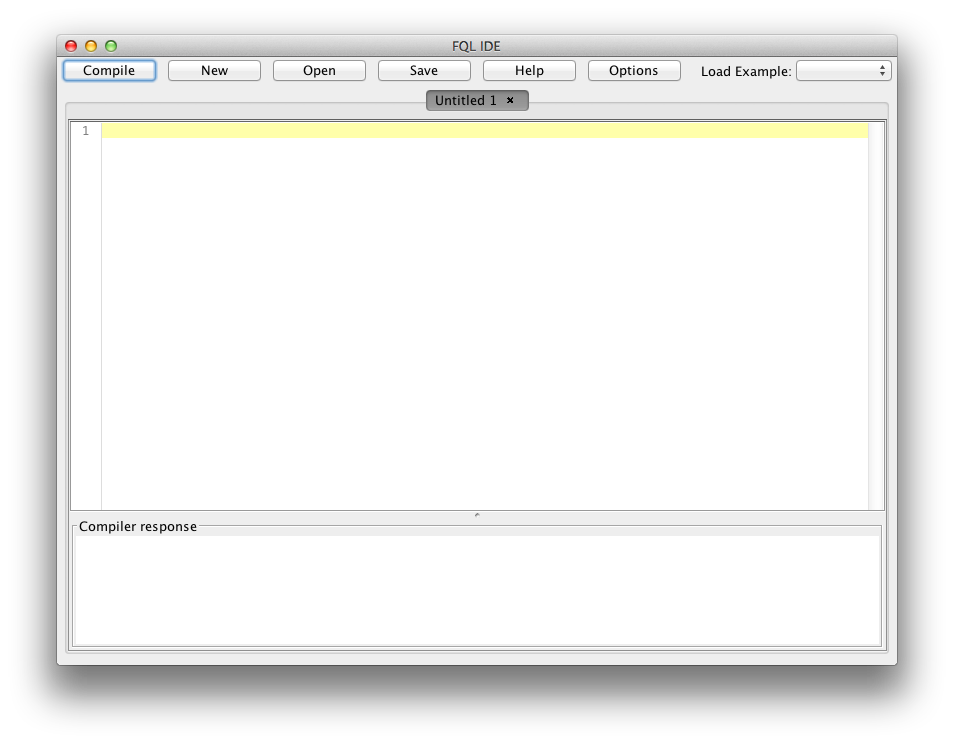
\includegraphics[width=5in]{initial}
%\end{center}

The AQL IDE contains a multi-tabbed text file editor that supports saving, opening, copy-paste, undo-redo, RTF export, code folding, outline-view, goto-definition, and search-replace through right-click context menus, menu bars, and keyboard shortcuts.  A variety of options are available in the options menu (text size, default file path, etc.)  Below each AQL text editor is a response text area that displays error and status messages.  The built-in AQL examples are loaded by selecting them from load-example combo-box in the upper-right of the IDE.  AQL programs are executed by pressing the run button in the upper-left of the IDE.  While an AQL program is running its status will be continually updated in the response area.  AQL programs that are running can be manually terminated using the abort menu option.   When an AQL program finishes running, the AQL IDE displays a graphical viewer allowing the result of the AQL program to be visually inspected.  Manual termination of AQL programs is best-effort and terminated AQL programs may leave resources (e.g., JDBC connections) open.

\section{Changing the Memory Limit}

To run the AQL IDE with more/less than the default 64mb heap, you must use a command line option such as:
\begin{verbatim}
java -Xms512m -Xmx2048m -jar aql.jar
\end{verbatim}

\section{Adding JDBC drivers to the classpath}

To run the AQL IDE with a particular JDBC driver requires placing the driver on the class path using a ``-cp'' command line option {\bf and} running java directly, for example:
\begin{verbatim}
java -cp "./mysql-connector-java-5.1.27-bin.jar:./aql.jar" catdata.ide.IDE 
\end{verbatim}

On some systems, especially windows systems, the colon in the classpath may need to be replaced with a semi-colon.

\section{Using AQL without a GUI}

The AQL IDE also supports command-line execution: an AQL program is passed to stdin, and an HTML view of the result is output on stdout:
\begin{verbatim}
java -cp "./aql.jar" catdata.aql.exp.AqlInACan.openCan
\end{verbatim}

\section{HTML markup}
The AQL IDE allows HTML markup to be inserted into AQL files.  After a program has compiled, the ``emit as HTML'' option in the AQL menu will emit the HTML code.  The HTML will contain pretty-printings of the program text, HTML tables for instances, and (possibly) javascript graphs for schemas.  To insert HTML, use the keyword {\tt html}, then brackets, then (*, and then a quoted string (note that because the HTML appears in a string, any quotes and backslashes within that string must be escaped).  For example,
\begin{verbatim}
instance I = ...

html { (* "<html>Hello world<a href=\"main.html\">link</a></html>" *) } 

instance J = ...
\end{verbatim}

The AQL tutorial, built-in as the Tutorial example, illustrates HTML output.  Alternatively, {\bf markdown} (a simplified way to write HTML) can be used; use the keyword {\tt md} instead of {\tt html}.  Note that AQL emits HTML tables that, when clicked, sort themselves by invoking javascript code from
\begin{verbatim}
https://categoricaldata.net/js/simple.js
\end{verbatim}
and a CSS style file is at
\begin{verbatim}
https://categoricaldata.net/css/simple.js
\end{verbatim}

\section{Just in time compilation}

The AQL IDE theorem provers benefit greatly from native compilation, which the JVM performs lazily.  Experiments suggest several AQL theorem provers become 2-4x faster after JIT compilation.  For this reason, if performance is critical it is suggested to run a few ``warm-up'' built-in examples to trigger JIT compilation.

\chapter{AQL Basics}

\section{Comments}

Comments in AQL are C style, either ``//'' or ``/* */''.  

\section{Kinds}

A {\it kind} is either {\it typeside}, {\it schema},  {\it instance}, (schema) {\it  mapping}, (instance) {\it transform}, {\it query}, {\it graph},  {\it pragma}, {\it schema\_colimit}, or {\it constraints}. 

\section{Identifiers}

AQL identifiers are case-sensitive alpha-numeric strings, or arbitrary strings escaped with double-quotes.

\section{Declarations}

An AQL program is an ordered list of {\it declarations} of the form $kind \ name = expression$.  Each declaration consists of a $name$, which is an   identifier unique per AQL program. Each $expression$ is evaluated by the AQL execution engine and the resulting artifact (a schema, instance, query, etc., according to $kind$) is bound to the declaration $name$.  Before execution, the AQL engine checks that a program has an acyclic set of dependencies.

\section{Caching}

The AQL IDE will cache result artifacts to save time in subsequent executions; this behavior can be disabled per-expression through the {\tt always\_reload} option.  Disabling caching is can be useful when an AQL program contains side-effecting pragmas.

\section{Terms}

An AQL program contains many {\it terms}.  Their raw syntax is:

\begin{verbatim}
<term> ::= <identifier> | <identifier>@<identifier> | <term> . <identifier>
              | (<term> <identifier> <term>) | <identifier>(<term>, ...) 
\end{verbatim}

Intuitively, terms denote ``things which can be named'' in typesides (java objects, functions and types), schemas (entities, attributes, foreign keys), and instances (generators and labelled nulls).  Their abstract syntax is: 
\begin{verbatim}
<term> ::= <variable> | <java object>@<type> | <generator> | <labelled null> 
              | <term>.<attribute> | <term>.<foreign key> | <function>(<term>, ...) 
\end{verbatim}

The syntax $p.q$ abbreviates $q(p)$.  Parenthesis in AQL cannot be added (e.g., if $v$ is a variable, then $(v)$ is not valid syntax) or omitted (e.g., $(x + y)$ cannot be written as $x + y$)..  

\section{Contexts}

An AQL program contains many {\it contexts}.  Let $K,V$ be two non-terminals in a grammar.  A context over $K,V$ is a (possibly empty) list of $K,V$ pairs:
\begin{verbatim}
<ctx>(K,V) ::= "" | K : V <ctx>
\end{verbatim} 

The syntax $a \ b \ c \ \ldots : X$ abbreviates the context $a:X \ b:X \ c:X$.  Occasionally, {\tt ->} or {\tt =} will be used in place of {\tt :} (e.g., in mappings).  With the exception of {\tt multi\_equations} in instance literals, lists (including contexts) are space-separated.

\section{Terms in Contexts}
The abstract syntax for a {\it term-in-context} is: 
\begin{verbatim}
<type-or-entity> ::= <type> | <entity>
<term-in-ctx> ::= ctx(<variable>,<type-or-entity>) . <term>
\end{verbatim}

Terms are subject to an intuitive typing discipline; e.g., if $f : Nat \to Nat$, then for $f(e)$ to be well-typed, it must be that $e : Nat$.

\section{Paths}
A {\it path} is a well-typed list of foreign keys. Paths give rise to families of terms: if $f_1, \ldots, f_k$ is a path, then for every term $e$, $f_k( \ldots f_1(e))$ is a term.

\section{Equations}
The abstract syntax for an {\it equation} is: 
\begin{verbatim}
<type-or-entity> ::= <type> | <entity>
<term-in-ctx> ::= forall ctx(<variable>,<type-or-entity>) . <term> = <term>
\end{verbatim}
The  type (or entity) of each term must match.  A {\it path equation} is an equation of terms that are paths terminating on a variable.

\section{Sections, Literals, Options}
\label{section10}

Many AQL expressions are written using {\it sections}. In the example below, {\tt imports}, {\tt types}, {\tt constants}, and {\tt options} are the sections.
\begin{verbatim}
typeside Ty = literal {
  imports
    Arithmetic
  types
    Bool
  constants
    t f : Bool	
  options
    timeout = 5  
}
\end{verbatim}
The type side $Ty$ is an example of a {\it literal}; i.e., an expression that evaluates to itself.  All AQL kinds except for pragmas have literals.  Literals are also called {\it constants}, but they should not be confused with the {\tt constants} declared in AQL type sides.  All sections are optional, but they must appear in the order specified in this manual. 

Many expressions contain lists of key-value pairs that specify options in an option section.  The defaults of these options many change with new releases of AQL and are displayed in the AQL pane of the AQL IDE options menu.  The effect of these options is described in the rest of the manual.  In the above example, the execution timeout for the type side is set to five seconds.  Every expression that supports options supports the timeout option, as well as the GUI (display) options and the always reload option.  

Every AQL file may contain an optional options section before the list of declarations.  These options are inherited by every expression (e.g., so you can set the timeout globally to 30 seconds, rather than having to specify that for every expression).  

\section{Imports}

Many literal expressions, including type sides, schemas, mappings, queries, instances, and transforms can contain {\tt import} sections.  Each import section must contain a list of names.  For example, a typeside $T$ can import another typeside $T'$, whose effect is the same as if $T'$ were {\it textually included} in $T$.  Almost always each imported name should be a literal or an identity.  In the above example (Section~\ref{section10}), $Ty$ imports the typeside for arithmetic.
 
\section{AQL's Typing Discipline}

Officially, AQL programs are nominally typed.  For example, if {\tt schema X = Y} is a declaration, then {\tt id X} has type {\tt X -> X} {\it which is not equal to} {\tt Y -> Y} (beause {\tt X} and {\tt Y} are different {\it names}).  Unofficially, the AQL type-checker accepts many programs that are not nominally typed but are still well-typed.

\section{Scripting with Side Effects using Pragmas}

All AQL expressions with the exception of pragmas are side-effect free.  Many pragmas have side effects; for example, {\tt export\_instance\_jdbc} can write data to a database via JDBC.  Therefore, the execution order for pragmas matters.  To establish an ordering, each pragma implicitly depends on all declarations before it.  Consequently, pragmas can bottleneck AQL execution (the AQL execution engine is multi-threaded).  Pragmas are provided to execute arbitrary SQL (via JDBC), Java (via Nashorn javascript), and command-line commands, thereby allowing AQL programs to ``script'' an entire data integration / ETL flow.

\section{Algebraic Databases are Deductive Databases}

AQL databases are deductive: that is, they are defined only up to provable equality.  This means, for example, that an instance may contain a row whose value is $2+2$ rather than $4$.  From AQL's perspective, $2+2$ and $4$ are freely interchangeable.  However, when exporting AQL databases to CSV or SQL, there is a difference between $2+2$ and $4$: the former is an expression, and the latter is a constant, and they can be exported differently.  To establish a true normal form (i.e., to everywhere prefer $4$ over $2+2$) it is necessary to use java type sides.

\section{Java (script) typesides and inline functions}

AQL typesides can contain bindings of types to java classes and of function symbols to javascript code.  (In this manual, we use java and javascript interchangeably, because the Java VM's Nashorn execution engine for javascript allows the use of java functions.)  The AQL execution engine will invoke this javascript code during execution, for example, to reduce $2+2$ to $4$.  In order to maintain completeness of AQL's theorem prover, certain equations involving java are disallowed.  This restriction can be overridden using the {\tt allow\_java\_eqs\_unsafe} option.  Java functions need to be side-effect free.  For SQL interaction, AQL provides a special built-in typeside called {\tt sql}.  

\section{Consistency}

It is possible for an AQL instance to be inconsistent; i.e., for $1 = 2$ to be provable.  If this behavior is not desired, consistency can be enforced using the {\tt require\_consistency} option.  This option is overly conservative: it may disallow instances that are consistent.

\section{Labelled Nulls}

Nulls in AQL are labelled; i.e., two null values need not be equal.  In addition, there is no way to test if a value is a labelled null.  Non-labelled nulls can be defined using optional types in typesides.  For example:

\begin{verbatim}
 types
   Nat NullableNat Bool
 functions
   null : NullableNat
   in : Nat -> NullableNat	
   out : NullableNat -> Nat
   isNull : NullableNat -> Bool
 equations
    forall x. out (in x) = x	
\end{verbatim}	

\section{Schema, Mapping, Query, Instance, Transform Inference}

The AQL IDE provides code-assistance functions.  For example, if $S$ and $T$ are schemas, then if {\tt literal : S -> T} is highlighted, the AQL editor is right-clicked, and ``infer mapping'' is selected in the resulting pop-up menu, then the IDE will add the skeleton of a mapping declaration.  In particular, it will list all of the entities, attributes, and foreign keys for $S$ and will describe how they can be mapped into $T$; and similarly for queries, transforms, etc.  In addition, by pressing control-shift-space after a kind name (e.g., typeside), the AQL editor will pop up a template containing the sections for a corresponding literal.

\section{Theorem Proving}

The AQL engine uses automated theorem proving technology to ensure that AQL programs cannot fail at runtime (modulo javascript errors), or materialize instances that do not satisfy their data integrity constraints.  To provide this guarantee, every AQL typeside, schema, and instance must be a decidable equational theory.  Not all equational theories are decidable; moreover, automated theorem proving methods can be slow or incomplete.  The AQL engine provides a number of theorem provers which by default it uses automatically as appropriate; however, specific theorem provers can be chosen by using the {\tt prover} option.  In addition, schema mappings and transforms and queries are required to preserve provable equality; this behavior can be disabled with the {\tt dont\_validate\_unsafe} option.  To find out which prover is being used, click the ``info'' button in the ``DP'' pane in the viewer.  The DP pane also allows users to decide the equality of arbitrary terms by entering them as text (useful for debugging AQL programs).

\section{Provenance / Lineage of generated IDs}

The AQL engine generates fresh IDs during execution.  These IDs are exported via JDBC and CSV and are used by the engine internally.  The AQL engine maintains a ``lineage'' for these IDs that is displayed in the AQL viewer.  This lineage is invariably more meaningful to humans than the generated IDs.  For example, rather than display ``fresh ID 847'', the viewer might display ``bill.manager''.  It is important to remember that these lineages are not canonical, are provided for convenience only, and the real data is the generated IDs, not the lineages.


%%%%%%%%%%%%%%%%%%%%%%%%%%%%%%%%%%%%%%%%%%%%%%

\chapter{Kind {\tt graph}}
AQL graphs are directed multi-graphs with labels on nodes and edges.

\section{{\tt literal}}
\subsection{{\tt imports}}
A list of names of {\tt graph}s.
\subsection{{\tt nodes}}
A list of identifiers.
\subsection{{\tt edges}}
A {\tt ctx(<edge>, <node> -> <node>)}.

\chapter{Kind {\tt typeside}}
Type sides contain types, function symbols (called constants when 0-ary), and equations, as well java bindings for certain types. 

\section{{\tt empty}}
The empty {\tt typeside} with no types or java types.

\section{{\tt typeSideOf <schema>}}
The {\tt typeside} that a {\tt schema} is on.

\section{{\tt sql}}
The {\tt typeside} with java types corresponding to SQL.

\section{{\tt literal : <typeside>}}
\subsection{{\tt imports}}
A list of names of {\tt typeside}s.
\subsection{{\tt types}}
A list of identifiers.
\subsection{{\tt constants}}
A {\tt ctx(<constant>, <type>)}.
\subsection{{\tt functions}}
A {\tt ctx(<function>, <type>, ... -> <type>)}.
\subsection{{\tt equations}}
A list of equations, i.e., a list of {\tt forall ctx(<variable>,<type>) . <term> = <term>}.  
\subsection{{\tt java\_types}}
A {\tt ctx(<java\_type>, [java class name])}.  
\subsection{{\tt java\_constants}}
A {\tt ctx(<java\_type>, [javascript code])}.  During parsing, the {\tt input[0]} of {\tt javascript code} is passed a string, and should return a java object of type {\tt java\_type}.
\subsection{{\tt java\_functions}}
A {\tt ctx(<java\_function>, <java\_type> , ... -> <java\_type> = [javascript code])}.  {\tt javascript code} receives its arguments as {\tt input[0] , ...}.
\subsection{{\tt options}}
Allowable options are {\tt timeout}, {\tt prover} and related options, and {\tt allow\_java\_eqs\_unsafe}.

\chapter{Kind {\tt schema}}

All schemas are ``on'' a typeside, and contain entities, foreign keys, attributes, and equations.

\section{{\tt empty : <typeside>}}
The empty {\tt schema} with no entities, foreign keys, or attributes, on a particular {\tt typeside}.

\section{{\tt schemaOf <instance>}}
The {\tt schema} of an {\tt instance}.

%\section{{\tt dom <mapping>}}
%%check
%The source of a schema mapping.
%
%\section{{\tt cod <mapping>}}
%%check
%The target of a schema mapping.
%
%\section{{\tt src <query>}}
%%check
%The source of a query.
%
\section{{\tt dst <query>}}
%%check
The target of a query.

\section{{\tt literal : <typeside>}}
\subsection{{\tt imports}}
A list of names of kind {\tt typeside}.
\subsection{{\tt entities}}
A list of identifiers.
\subsection{{\tt foreign\_keys}}
A {\tt ctx(<foreign\_key>, <entity> -> <entity>)}.
\subsection{{\tt path\_equations}}
A list of path equations, where each path starts and ends at an entity.
\subsection{{\tt attributes}}
A {\tt ctx(<function>, <entity> -> <type>)}.
\subsection{{\tt observation\_equations}}
A list of {\tt forall <variable> : <entity> . <term> = <term> }, where the terms are of the same type (not entity).  Alternatively, equations of the form $\forall x. \ p(x) = q(x)$, where $p,q$ are paths, can simply be written as $p = q$.

\subsection{{\tt options}}
Allowable options are {\tt timeout}, {\tt prover} and related options, and {\tt allow\_java\_eqs\_unsafe}.

\section{{\tt getSchema <schema\_colimit>}}

Gets the schema associated with a colimit of schemas.

\chapter{Kind  {\tt mapping}}

A schema mapping $F : S \to T$ takes entities in $S$ to entities in $T$, foreign keys in $S$ to paths in $T$, and attributes in $S$ to terms in $T$, in a way that is functorial: if $f : s \to s'$ is a symbol in $S$, then it must be that $F(f) : F(s) \to F(s')$.  In addition, if $\forall \Gamma . e = e'$ is provable in $S$, then $\forall F(\Gamma). F(e) = F(e')$ must be provable in $T$.

\section{{\tt id <schema>}}
The identity schema mapping on a particular schema.

\section{{\tt [<mapping> ; <mapping>]}}
Composes two mappings: if {\tt f : A -> B} and {\tt g : B -> C}, then {\tt (f ; g) : A -> C}.

\section{{\tt literal : <schema1> -> <schema2>}}
\subsection{{\tt imports}}
A list of names of kind {\tt mapping}.
\subsection{{\tt entities}}
A {\tt ctx(<entity1>, <entity2>)}.
\subsection{{\tt foreign\_keys}}
A {\tt ctx(<foreign\_key1>, <path2>)}.  
\subsection{{\tt attributes}}
A {\tt ctx(<attribute1>, lambda x:<entity>. <term> : <type> )}, where {\tt type} is the type of {\tt attribute1} and $x$ occurs free in {\tt term}.  Any variable can be used in place of $x$.  Alternatively, attribute mappings of the form $\lambda x. \ x.p$, where $p$ is a path, can simply be written as $p$.

\subsection{{\tt options}}
Allowable options are {\tt timeout} and {\tt dont\_validate\_unsafe}, which disables checking that equations preserved.

\chapter{Kind  {\tt query}}
A query $S \to T$ assigns to each entity $en$ in $S$ a (``frozen'') instance on $T$, which we will write as $[en]$, and to each foreign key $fk : e \to e'$ a transform $[fk] : [e'] \to [e]$ (note the reversal), and to each attribute $att : e \to \tau$ a term of type $\tau$ in context $[e]$.  

\section{{\tt id <schema>}}
The identity query on a schema.

\section{{\tt toQuery <mapping>}}
Constructs the query $Q^F$ such that $eval(Q^F) \cong \Delta_F$ and $coeval(Q_F) \cong \Sigma_F$ for the mapping F.

\section{{\tt toCoQuery <mapping>}}
Constructs the query $Q_F$ such that $coeval(Q_F) \cong \Delta_F$ and $eval(Q_F) \cong \Pi_F$ for the mapping F.  The option {\tt toCoQuery\_max\_term\_size} controls the maximum size of the terms to be searched.

\section{{\tt [ <query> ; <query> ]}}
Composes two queries: if {\tt f : A -> B} and {\tt g : B -> C}, then {\tt [ f ; g ] : A -> C} using the complete ``view unfolding'' algorithm.   The incomplete co-evaluation based method can be used instead with the {\tt query\_compose\_use\_incomplete} option.

\section{{\tt literal : <schema> -> <schema>}}
\subsection{{\tt imports}}
A list of names of queries.
\subsection{{\tt entities}}
A {\tt ctx(<entity>, <instance>, ctx(<attribute>, <term>))}.  The instance uses keywords {\tt from} and {\tt where} instead of {\tt generators} and {\tt equations}.  Note that only only generators, not labelled nulls, can be used in the instance (i.e., {\tt from} $\ v:Integer \ $ is not allowed).  Associated with each entity is a context mapping attributes to terms (the {\tt return} clause).

\subsection{{\tt foreign\_keys}}
A {\tt ctx(<foreign key>, <transform>)}.

\subsection{{\tt options}}
Allowed are {\tt timeout} and {\tt dont\_validate\_unsafe}.  Note that each instance and transform in the query can have its own options.  See the {\tt query}-prefixed options.

\section{{\tt simple : <schema>}} 

\subsection{{\tt entities}}
A {\tt <instance>, ctx(<attribute>, <term>)}, i.e., a single from/where/return (sub) query of the form found in the {\tt literal} queries.  The target schema associated with these simple one-table queries has one entity and the attributes are generated automatically by the return clause. 

\section{{\tt getMapping <schema\_colimit> <schema>}}

The expression ${\tt getMapping} \ C \ X$ gets the mapping $X \to C$ associated with schema $X$ in the colimit of schemas $C$.

\chapter{Kind {\tt constraints}}

\section{{\tt literal : <schema>}}

A set of constraints (embedded dependencies). 

\subsection{{\tt imports}}
A list of constraints names.

\subsection{{\tt constraints}}
 Each constraint has the form
\begin{verbatim}
forall x1 : E1 , ..., xN : En 
where p = q  p' = q' ...
->
exists y1:E'1, ..., yM : E;m 
where p'' = q''  p''' = q''' ...
\end{verbatim}

\subsubsection{{\tt forall}}
A {\tt ctx(<generator> , <entity>)}.

\subsubsection{{\tt where}}
A list of ground (non quantified) equations.

\subsubsection{{\tt exists}}
A {\tt ctx(<generator> , <entity>)}.  Optionally, {\tt exists unique} can be used instead.

\subsubsection{{\tt where}}
A list of ground (non quantified) equations.

\chapter{Kind {\tt instance}}
\section{{\tt empty : <schema>}}
The empty instance with no generators or labelled nulls on a particular schema.

\section{{\tt src <transform>}}
The source of a transform.

\section{{\tt dst <transform>}}
The target of a transform.

\section{{\tt distinct <instance>}}
Returns an instance that equates all (entity) generators that are observationally equivalent (i.e., are provably equal on all attributes and foreign keys) in the input instance.  

\section{{\tt eval <query> <instance>}}
Evaluates a query on an instance.  If $Q : S \to T$, and $I$ is an instance on $S$, then $eval \ Q \ I$ is an instance on $T$.
See the {\tt eval}-prefixed options.

\section{{\tt coeval <query> <instance>}}
Co-evaluates a query on an instance.  If $Q : S \to T$, and $J$ is an instance on $T$, then $coeval \ Q \ J$ is an instance on $S$.
\subsection{\tt options}
Allowed options are {\tt timeout} and {\tt prover} and related options.

\section{{\tt delta <mapping> <instance>}}
If $F : S \to T$ is a mapping and $J$ is an $T$-instance, then $\Delta_F J$ is an $S$-instance. 

\section{{\tt sigma <mapping> <instance>}}
If $F : S \to T$ is a mapping and $I$ is an $S$-instance, then $\Sigma_F I$ is a $T$-instance. 

\section{{\tt coproduct\_sigma (<mapping> <instance>)+ : <schema>}}
The expression {\tt coproduct\_sigma}  $F \ I \ G \ J \ : S$ means $\Sigma_F(I) + \Sigma_G(J)$, where $+$ is $S$-instance co-product.  Arbitrarily many mapping-instance pairs can be used.  This operation is provided to help minimize the number of intermediate materializations required to execute an AQL program.

\section{{\tt coproduct <instance> + ... + <instance> : <schema>}}
Takes the coproduct of the input instances.  Desugars into {\tt coproduct\_sigma} along the identity mapping.

\section{{\tt coproduct\_unrestricted <instance> + ... + <instance> : <schema>}}
Takes the coproduct of the input instances.  Note that the instances must be names; unlike the other coproduct expressions, there is no requirement that generators not overlap in this expression.

\section{{\tt coequalize <transform> <transform>}}
Computes the coqualizer of two transforms.


\section{{\tt colimit <graph> : <schema>}}
Let $G$ be a graph and $S$ a schema.

\subsection{{\tt nodes}}
A list of names of {\tt instance}s on schema $S$.

\subsection{{\tt edges}}
A {\tt ctx(<name>, <transform>)}, where the transforms are typed according to the {\tt node} assignments.

\subsection{{\tt options}}
Allowable options are {\tt timeout} and {\tt static\_typing}, which when disabled causes AQL to type check the colimit at runtime rather than compile time.  This will reduce the number of transforms required to compute any particular colimit, at the cost of potential runtime failure.

\section{{\tt import\_jdbc [jdbcclass] [jdbcuri] : <schema>}}

\subsection{entities}
A {\tt ctx(<entity> | <attribute> | <foreign key> | <type> , [sql code])}.  The SQL code for each entity should return a table with an ID column and one column per attribute/foreign key from that table.  (See the {\tt import\_joined} option for an alternative inpurt format.). Note that these tables must be complete: this keyword imports a model (set of tables) of a schema, not a presentation of a model of a schema (i.e., as {\tt literal} does).  To import an instance as a theory, use the {\tt import\_as\_theory} option.  When the [jdbcclass] and [jdbcuri] are the empty string, their values will be determined by the {\tt jdbc\_default\_class} and {\tt jdbc\_default\_string} options. 

\subsection{{\tt options}}
Allowed are {\tt timeout}, {\tt prover} and related options, {\tt always\_reload}, and {\tt require\_consistency}.  


\section{{\tt quotient\_jdbc [jdbcclass] [jdbcuri] <instance>}}
Expects a list of (single) SQL commands inside a section.  Each SQL query should return a 2 column table, where each column has a generator from the input instance.  The union of these tables defines an equivalence relation and this expression quotients the input instance by this relation.  When the [jdbcclass] and [jdbcuri] are the empty string, their values will be determined by the {\tt jdbc\_default\_class} and {\tt jdbc\_default\_string} options.

\section{{\tt quotient\_csv <instance>}}
Expects a list of filenames inside a section.  Each file should have 2 columns, where each column has a generator from the input instance.  The union of these files defines an equivalence relation and this expression quotients the input instance by this relation. 

\section{{\tt import\_jdbc\_all [jdbcclass] [jdbcuri]}}

Imports a SQL database onto an autogenerated AQL schema.  The AQL schema will have one attribute per column in the input DB, and one foreign key per foreign key in the input DB, and equations capturing the input DB's foreign key constraints.  The type side will have a single type, ``dom''.  When the [jdbcclass] and [jdbcuri] are the empty string, their values will be determined by the {\tt jdbc\_default\_class} and {\tt jdbc\_default\_string} options.

\subsection{{\tt options}}
Allowed are {\tt timeout}, {\tt prover} and related options, {\tt always\_reload}, {\tt require\_consistency}, and {\tt schema\_only} (imports the empty instance).

\section{{\tt import\_csv [directory] : schema}}
%\subsection{entities}
A {\tt ctx(<string> | [string])}.  For each entity $en$, expects a file $en$.csv in the directory.  The file extension can be changed with the {\tt csv\_file\_extension} option.  The file for $en$ should be a CSV file with a header; the fields of the header should be an ID column name (specified using options), as well as any attributes and foreign keys whose domain is $en$.  The mapping between the schemas entities (ID columns), attributes, and foreign keys and the headers of the CSV file are controlled by the section; see the CSV built-in example for details.

Records can contain nulls (using the string specified in options).  Note that these tables must be complete: this keyword imports a model (set of tables) of a schema, not a presentation of a model of a schema (i.e., as {\tt literal} does).  To import an instance as a theory, use the {\tt import\_as\_theory} option.  To auto generate IDs, see {\tt csv\_generate\_ids} option.

\subsection{{\tt options}}
Allowed are {\tt timeout}, {\tt prover} and related options, {\tt always\_reload}, {\tt csv} related options, {\tt id\_column\_name}, and and {\tt require\_consistency}. 


\section{{\tt literal : <schema>}}

An instance is a collection of generators at entities and labelled nulls at types, as well as ground equations.

\subsection{{\tt imports}}
A list of instance names.

\subsection{{\tt generators}}
A {\tt ctx(<generator> | <labelled null>, <entity> | <type>)}.

\subsection{{\tt equations}}
A list of ground (non quantified) equations.

\subsection{{\tt multi\_equations}}
A {\tt ctx(<attribute> | <foreign key>, {<generator> <labelled null>, ... }}.  For example,
\begin{verbatim}
multi\_equations
	name -> {person1 bill, person2 alice}
\end{verbatim}
is equivalent to
\begin{verbatim}
equations
	person1.name = bill
	person2.name = alice
\end{verbatim}
The key-value pairs in multi-equations must be comma separated (necessary for readability and error correction).

\subsection{{\tt options}}
Allowable options are {\tt timeout}, {\tt prover} and related options, {\tt require\_consistency}, and {\tt interpret\_as\_algebra}, which interprets the instance as a model, similar to JDBC / CSV import.  This behavior can be useful when writing down an instance that is already saturated and for which one wants to check the schema constraints, rather than impose them. See employees example.

\section{{\tt quotient : <instance>}}

\subsection{{\tt equations}}
A list of ground (non quantified) equations to quotient by.  Allowable options are {\tt timeout}, {\tt prover} and related options, and {\tt require\_consistency}.

\section{{\tt chase <constraints> <instance> [number]}}

Chases the input instance with the input constraints up to a maximum number of iterations.  If the chase succeeds, the result instance will satisfy the constraints.

\subsection{{\tt options}}
Allowable options are the same as for an instance.


\section{{\tt random : <schema>}}

Constructs a random instance with the specified number of generators per entity or type. Then for each generator $e:s$ and fk/att $f : s \to t$, it adds equation $f(e) = y$, where $y:t$ is a randomly selected generator (or no equation if t has no generators).

\subsection{{\tt generators}}
A {\tt ctx(<generator> | <labelled null> -> integer)}.

\subsection{{\tt options}}
Allowable options are the same for literal instances, and {\tt random\_seed}.

\chapter{Kind {\tt transform}}
\section{{\tt id <instance>}}
%todo
The identity transform on an instance.
\section{{\tt [<transform> ; <transform>]}}
%todo
Composes two transforms: if {\tt f: A -> B} and {\tt g: B -> C}, then {\tt (f ; g): A -> C}.

\section{{\tt distinct <transform>}}
If $t : I \to J$ is a transform, then $distinct \ t : distinct \ I \to distinct \ J$ is a transform.

\section{{\tt delta <mapping> <transform>}}
If $t : I \to J$ is a transform and $F$ a well-typed mapping, then $\Delta_Ft : \Delta_F(I) \to \Delta_F(J)$ is a transform.

\section{{\tt sigma <mapping> <transform>}}
If $t : I \to J$ is a transform and $F$ a well-typed mapping, then $\Sigma_Ft : \Sigma_F(I) \to \Sigma_F(J)$ is a transform.
\subsection{options1}
Passed to $\Sigma_F(I)$.
\subsection{options2}
Passed to $\Sigma_F(J)$.

\section{{\tt eval <query> <transform>}}
If $t : I \to J$ is a transform, and $Q$ a well-typed query, then $eval_Qt : eval_Q(I) \to eval_Q(J)$ is a transform.

\section{{\tt coeval <query> <transform>}}
If $t : I \to J$ is a transform, and $Q$ a well-typed query then $coeval_Qt : eval_Q(I) \to eval_Q(J)$ is a transform.
\subsection{options1}
Passed to $coeval_Q(I)$.
\subsection{options2}
Passed to $coeval_Q(J)$.

\section{{\tt unit <mapping> <instance>}}
If $F : S \to T$ is a schema mapping and $I$ is an $S$ instance, then $unit_F(I) : I \to \Delta_F(\Sigma_F(I))$.
\subsection{options}
Passed to $\Sigma_F(I)$.

\section{{\tt counit <mapping> <instance>}}
If $F : S \to T$ is a schema mapping and $J$ is an $T$ instance, then $counit_F(J) : \Sigma_F(\Delta_F(J))  \to J$.
\subsection{options}
Passed to $\Sigma_F(\Delta_F(J))$.

\section{{\tt unit\_query <query> <instance>}}
If $Q : S \to T$ is a query and $J$ is a $T$ instance, then $unit_Q(I) : eval_Q(coeval_Q(J)) \to J$.
\subsection{options}
Passed to $coeval_Q(IJ)$.

\section{{\tt counit\_query <query> <instance>}}
If $Q : S \to T$ is a query and $I$ is an $S$ instance, then $counit_Q(I) : coeval_Q(eval_Q(I))  \to I$.
\subsection{options}
Passed to $coeval_Q(eval_Q(I))$.

\section{{\tt import\_jdbc  [jdbcclass] [jdbcuri] : <instance> -> <instance>}}
Imports a transform using JDBC. When the [jdbcclass] and [jdbcuri] are the empty string, their values will be determined by the {\tt jdbc\_default\_class} and {\tt jdbc\_default\_string} options.

\subsection{entities}
A {\tt ctx(<entity> | [sql code])} section assigns each entity $en$ to a SQL query.  The first column is interpreted as the source and the second column as the target.

\subsection{options}
Allowed are {\tt timeout}, {\tt always\_reload}.  

\section{{\tt import\_csv [filename] : <instance> -> <instance>}} 

Imports a transform from CSV.  

\subsection{entities}
A {\tt ctx(<entity> | [filename])} section assigns each entity $en$ to a file.  The first column is interpreted as the source and the second column as the target.


\subsection{options}
Allowable options are {\tt timeout} and {\tt always\_reload}  and {\tt csv} related options. 

\section{{\tt literal : <instance> -> <instance>}}

\subsection{{\tt generators}}
A {\tt ctx(<generator> | <labelled null>, <term>)} that preserves types.  Note that the {\tt term} must be ground (not in a context).  

\subsection{{\tt options}}
Allowed are {\tt transform} and {\tt dont\_validate\_unsafe}.

\chapter{Kind {\tt pragma}}
\section{{\tt exec\_cmdline}}
Expects a list of strings inside a section.  Each string will be executed by the Java VM as an external process.  The return value of each command is displayed in the viewer.

\subsection{{\tt options}}

Allowable options are {\tt timeout} and {\tt always\_reload}.

\section{{\tt exec\_js}} 
Expects a list of strings inside a section.  Each string will be executed by the Java VM's Nashorn javascript execution engine.  The return value of each command is displayed in the viewer.

\subsection{{\tt options}}

Allowable options are {\tt timeout} and {\tt always\_reload}.

\section{{\tt exec\_jdbc [jdbcclass] [jdbcuri]}}
Expects a list of (single) SQL commands inside a section.  Each string will be executed by JDBC.  The return value of each command is displayed in the viewer.  When the [jdbcclass] and [jdbcuri] are the empty string, their values will be determined by the {\tt jdbc\_default\_class} and {\tt jdbc\_default\_string} options.

\subsection{{\tt options}}

Allowable options are {\tt timeout} and {\tt always\_reload}.

\section{{\tt check <constraints> <instance>}}

Checks that an instance obeys a set of constraints.

\section{{\tt assert\_consistent <instance>}}

Conservatively checks that an instance is consistent (e.g., does not prove $1=2$) by checking that it has a free type algebra.

%%%%%%%%%%

\section{{\tt export\_csv\_instance [jdbcclass] [jdbcuri] <instance>}} 

Exports an instance as CSV.  The directory name will contain one file named $en.csv$ per entity $en$, and if non-empty, one file named $t.csv$ per type $t$.  The file for $en$ will be a CSV file with a header; the fields of the header will be an ID column name (specified using options), as well as any attributes and foreign keys whose domain is $en$.   AQL rows that are not constants will be exported as nulls.

\subsection{{\tt options}}
Allowed are {\tt timeout}, {\tt always\_reload}, {\tt csv} related options, and {\tt id\_column\_name}, and {\it start\_ids\_at}.

%%
\section{{\tt export\_csv\_transform [filename] <transform>}}

Exports a transform as CSV.  The filename will be a CSV file without a header and with two columns (src, tgt).  

\subsection{options1}
Allowable options are {\tt timeout} and {\tt always\_reload}  and {\tt csv} related options, and {\tt start\_ids\_at}.  Note that {\tt start\_ids\_at} is not inherited from the source instance.

\subsection{options1}
Allowable options are {\tt timeout} and {\tt always\_reload}  and {\tt csv} related options, and {\it start\_ids\_at}.  Note that {\tt start\_ids\_at} is not inherited from the source instance.

%%%%%%%%%%%
\section{{\tt export\_jdbc\_instance <instance> [jdbcclass] [jdbcuri] [prefix] }}

Exports an instance (on SQL typeside) using JDBC.  There will be a table $prefixen$ for each entity $en$.  The columns will be the attributes and foreign keys whose domain is $en$, and an ID column whose name is set in options.  AQL rows that are not constants will be exported as NULL.  When the [jdbcclass] and [jdbcuri] are the empty string, their values will be determined by the {\tt jdbc\_default\_class} and {\tt jdbc\_default\_string} options, and {\tt start\_ids\_at}.

\subsection{options}
Allowable options are {\tt timeout}  and {\tt always\_reload} and  {\tt id\_column\_name} and {\tt varchar\_length}.

\section{{\tt export\_jdbc\_query <query> [jdbcclass] [jdbcuri] [prefixSrc] [prefixDst] }}

Exports a query (on SQL typeside) as a set of views using JDBC.  There will be a view $prefixen$ for each entity $en$.  The columns will be the attributes and foreign keys whose domain is $en$, and an ID column whose name is set in options.  When the [jdbcclass] and [jdbcuri] are the empty string, their values will be determined by the {\tt jdbc\_default\_class} and {\tt jdbc\_default\_string} options.

\subsection{options}
Allowable options are {\tt timeout}  and {\tt always\_reload} and  {\tt id\_column\_name} and {\tt varchar\_length}.


%%

\section{{\tt export\_jdbc\_transform [jdbcclass] [jdbcuri] [prefix] <transform>}}
Exports a transform using JDBC.  There will be a two-column table $prefixen$ for each entity $en$.  The two columns will be $srcidcol$ and $dstidcol$, where $idcol$ is the ID column name set in the options.   When the [jdbcclass] and [jdbcuri] are the empty string, their values will be determined by the {\tt jdbc\_default\_class} and {\tt jdbc\_default\_string} options.

\subsection{options1}
Allowed are {\tt timeout}, {\tt always\_reload},  {\tt id\_column\_name} and {\tt varchar\_length}, and {\tt start\_ids\_at}.  Note that {\tt start\_ids\_at} is not inherited from the source instance.
\subsection{options2}
Allowed are {\tt timeout}, {\tt always\_reload},  {\tt id\_column\_name} and {\tt varchar\_length, and {\tt start\_ids\_at}}.  Note that {\tt start\_ids\_at} is not inherited from the target instance.

\chapter{{\tt schema\_colimit}}

\section{{\tt quotient <schema> + ... + <schema> : <typeside>}}

Constructs a colimit of schemas as a quotient of a co-product.  Each schema must be a variable, whose name will serve as a prefix for attributes and foreign keys in the resulting colimit schema.  For this reason, the variable names must be distinct.  The entities of the resulting colimit schema are canonicalized strings describing equivalence classes of source entities.

\subsection{{\tt entity\_equations}}

Each equation has the form $v_1.e_1 = v_2.e_2$, where $v_1, v_2$ are schema names and $e_1, e_2$ are entities in $v_1, v_2$, respectively.

\subsection{{\tt path\_equations}}

Each equation has the form {\tt <path>=<path>}, where the foreign keys in each path have the form $v\_fk$, where $v$ is a schema name and $fk$ is a foreign key in $v$.  Note that the underscore used here is different than the period used in the preceding section; this discrepancy is required for AQL to have an unambiguous grammar.

\subsection{{\tt observation\_equations}}

Each equation has the form {\tt forall x. <term> = <term>}, where the symbols in each term have the form $v\_f(\ldots)$, where $v$ is a schema name and $f$ is a symbol in $v$.   Alternatively, equations of the form $\forall x. \ p(x) = q(x)$, where $p,q$ are paths, can simply be written as $p = q$.

\section{{\tt coproduct <schema> + ... + <schema> : <typeside>}}

Constructs a degenerate colimit of schemas as a co-product. 

\section{\tt modify <schema\_colimit>}

\subsection{{\tt rename entities}}
A $Ctx(name,name)$ specifying a renaming of entities.

\subsection{{\tt rename foreign\_keys}}
A $Ctx(name,name)$ specifying a renaming of foreign keys. 

\subsection{{\tt rename attributes}}

A $Ctx(name,name)$ specifying a renaming of attributes. 

\subsection{{\tt remove foreign\_keys}}

A $Ctx(name,path)$ specifying that the foreign key named by name can be deleted by replacing all occurrences of it by the given path.  AQL checks if the removal is semantics-preserving. 

\subsection{{\tt remove attributes}}

A $Ctx(name,\lambda x. \ term)$ specifying that the attribute named by name can be deleted by replacing all occurrences of it by the given term.  AQL checks if the removal is semantics-preserving. 
		
\section{{\tt wrap <schema\_colimit> <mapping> <mapping>}}
In $wrap X F G$, $F$ and $G$ must be inverses, and the result is the image of $X$ under $F$.
		
\chapter{{\tt options}}

\section{{\tt num\_threads = integer}}
Sets the number of threads to be used when running an AQL program.

\section{{\tt random\_seed = integer}}
Sets the random number generator seed.

\section{{\tt timeout = number (seconds)}}
Causes execution to halt after {\tt number} seconds.

\section{{\tt require\_consistency = boolean}}
When enabled, requires AQL instances to be consistent (e.g., to not prove 1=2).  (This is checked at runtime.)

\section{{\tt schema\_only = boolean}}

Used with {\tt import\_jdbc\_all} to import no data (only schema).

\section{{\tt static\_typing = boolean}}
When disabled, relaxes AQL's nominal typing discipline for colimit instances.

\section{{\tt allow\_java\_eqs\_unsafe = boolean}}
When enabled, allows arbitrary equations involving java typeside symbols.

\section{{\tt dont\_validate\_unsafe = boolean}}
When enabled, mappings and transforms and queries are not checked to be equality-preserving.  For a query, when true it also disables decision procedure construction for sub-queries.

\section{{\tt always\_reload = boolean}}
When enabled, pragmas (which can have side effects, like loading data from CSV files) are always executed and are not cached between runs of the AQL program.

\section{Import options}
%\subsection{{\tt csv\_charset = string}}
%Sets the java character set to be used for CSV import/export.  Should be one of 
%US-ASCII, 	
%ISO-8859-1,  	
%UTF-8, 	
%UTF-16BE,	
%UTF-16LE, 	
%UTF-16.
%
%\subsection{{\tt csv\_line\_delim\_string = string}}
%Sets the line delimiter for use in CSV import/export.

\subsection{{\tt csv\_field\_delim\_char = char}}
Sets the field delimiter for use in CSV import/export.

\subsection{{\tt csv\_escape\_char = char}}
Sets the escape character for use in CSV import/export.

\subsection{{\tt csv\_quote\_char = char}}
Sets the quote character for use in CSV import/export.

\subsection{{\tt csv\_file\_extension}}
Sets the file extension to expect during CSV import.

\subsection{{\tt csv\_generate\_ids}}
If no ID column is found, then AQL will create IDs during CSV import.

%
%\subsection{{\tt csv\_format = string}}
%Sets the Apache Commons CSV format to use.  Should be one of 
%    DEFAULT,
%    EXCEL,
%    MYSQL,
%    RFC4180,
%    TDF.

%
%\subsection{{\tt csv\_null\_string = string}}
%
%Sets the string that indicates null fields for use in CSV import/export.
%
\section{{\tt id\_column\_name = string}}
Specifies the name of the ID columns for CSV and JDBC import/export.

\section{{\tt varchar\_length = number}}
Specifies the length of the VARCHAR fields to use for JDBC export.

\section{ {\tt start\_ids\_at = integer}}

Specifies the integer to use as the initial integer when exporting data.

\section{ {\tt import\_as\_theory = boolean}}

\section{ {\tt jdbc\_default\_class = string } }

This string will be used in JDBC-related expressions when the JDBC driver class is the empty string.

\section{ {\tt jdbc\_default\_string = string } }

This string will be used in JDBC-related expressions when the JDBC string is the empty string.

When enabled, imported data will be interpreted as an equational theory, rather than an entire model.  This allows the importation of partial data sets, at the expense of additional theorem proving.
				
\section{{\tt dont\_verify\_is\_appropriate\_for\_prover\_unsafe = boolean}}
Many provers require that their input equational theories have a certain form (e.g., be unary).  When this option is enabled, this (possibly expensive) condition will not be checked.
				
\section{{\tt prover = string}}
Specifies which theorem prover to use.  The prover string should come from the list below.  Only the completion method has options.  Note that these theorem proving methods are not ``java aware''; to use java typesides, instances ``wrap'' these provers with java simplification.

\subsection{{\tt auto}}

The auto theorem proving method attempts the free, congruence, monoidal, and program methods, in that order.

 \subsection{{\tt fail}}
 
 Applies to all theories.  Always fails with an exception.
 
  \subsection{{\tt free}}
  
  Applies only to theories without equations.  Returns the syntactic equality of two terms.

\subsection{{\tt saturated}}

  Applies only to ground (variable-free) theories with a complete set of equations (e.g., as results from importing a CSV file).

\subsection{{\tt congruence}}

 Applies only to ground (variable-free theories).  Uses the classical congruence-closure with union-find algorithm.

\subsection{{\tt monoidal}}

Applies only to theories where all symbols are 0-ary or 1-ary.  Uses length-reducing Knuth-Bendix completion specialized to semi-Thue systems.

\subsection{{\tt program}}

Applies only to weakly orthogonal theories.  Interprets all equations $p = q$ as rewrite rules $p \to q$ if $p$ is syntactically smaller than $q$ and $q \to p$ if $q$ is syntactically smaller than $p$ and symbolically evaluates terms to normal forms.  Fails if an equation cannot be oriented.

\subsubsection{{\tt program\_allow\_nontermination\_unsafe}}

Interprets all equations $p = q$ as rewrite rules $p \to q$ regardless of termination behavior.  Can diverge.

\subsection{{\tt completion}}

Applies unfailing (ordered) Knuth-Bendix completion specialized to lexicographic path ordering.  If no completion precedence is given, attempts to infer a precedence using constraint-satisfaction techniques.

\subsubsection{{\tt completion\_precedence = list of strings}}

Defines the precedence to be used for Knuth-Bendix completion.  The list {\tt a b c} indicates that $a < b < c$.  Every symbol in a typeside or schema or instance must appear exactly once in this list.

\subsubsection{{\tt completion\_sort = boolean}}

Sorts the list of critical pairs in Knuth-Bendix completion by length, processing shorter pairs first (but still fairly).

\subsubsection{{\tt completion\_compose = boolean}}

Uses the ``compose'' inference rule in Knuth-Bendix completion.

\subsubsection{{\tt completion\_filter\_subsumed = boolean}}

Filters out equations that are substitution instances of other equations in Knuth-Bendix completion.

\subsubsection{{\tt completion\_syntactic\_ac = boolean}}

Enables special support for associative and commutative operators in Knuth-Bendix completion.

\section{GUI options}

Associated with each object is a {\it size}, according to its kind:
\begin{itemize}
\item pragma, constraints: length of the text string
\item instance: rows in the algebra
\item colimit schema: size of the schema
\item graph: nodes + edges
\item typeside: types + functions + equations
\item schema: entities + attributes + fks + equations
\item mapping, transform, query: size of source
\end{itemize}

The maximum size of such an object to be displayed in the viewer is controlled by the three options below.

\subsection{{\tt gui\_max\_table\_size = integer}}

For instances.

\subsection{{\tt gui\_max\_graph\_size = integer}}

For type sides, (colimit) schemas, mappings, transforms, queries.

\subsection{{\tt gui\_max\_string\_size = integer}}

For pragmas and constraints.

\subsection{{\tt gui\_rows\_to\_display = integer}}

Sets the maximum number of rows to display per table per instance in the viewer.  (I.e., the table in the viewer is conceptually similar to a SQL LIMIT query for the given number of rows).

\section{Evaluation options}

\subsection{{\tt eval\_max\_temp\_size = integer}}

Sets the maximum size of intermediate tables when executing sub-queries.

\subsection{{\tt eval\_reorder\_joins = boolean}}

Sets whether or not it is permissible for AQL to choose a join order based on exhaustive order enumeration under a heuristic cost metric.

\subsection{{\tt eval\_max\_plan\_depth = integer}}

If enabled, join reordering will be performed on FROM clauses with a number of variables smaller than this number (used to prevent the join ordering chooser from spending forever enumerating huge spaces of plans).

\subsection{{\tt eval\_join\_selectivity = float}}

Sets the join selectivity factor used by the cost metric heuristic for the join order chooser.

\subsection{{\tt eval\_use\_indices = boolean}}
			
Sets whether AQL should automatically index instances along their foreign keys and attributes, to reduce the number of intermediate tuples generated during query evaluation.
Also applies to SQL-based execution method.

\subsection{{\tt eval\_use\_sql\_above = integer}}

If possible, translate AQL queries into SQL and use AQL's built-in SQL database (``H2'')) to execute the query.  The translation process incurs overhead, so this option controls how large input instances have to be before translation is used.

\subsection{{\tt eval\_approx\_sql\_unsafe = boolean}}

Queries executed against instances containing nulls cannot be implemented by translation to SQL due to differences between null semantics in AQL and SQL.  
When enabled, AQL will execute the generated SQL anyway, leading to an undefined, but quickly computed, answer.  

\subsection{{\tt eval\_sql\_persistent\_indices = boolean}}

Queries executed by translation to SQL can store any computed indicies for future use. 

\section{{\tt query\_remove\_redundancy = boolean}}

Sets whether redundant joins (i.e., containing a binding $v$ and an equation $v = e$ where $v \notin e$) should be eliminated.
\section{Coproduct options}

The generators and labelled nulls of instances participating in a coproduct are required to be unique.  The following two options disable the uniqueness check.  These options are marked unsafe because they can result in an instance that is not a coproduct, but is rather a coproduct followed by a quotient.

\subsection{{\tt coproduct\_allow\_type\_collisions\_unsafe = boolean}}

\subsection{{\tt coproduct\_allow\_entity\_collisions\_unsafe = boolean}}

\subsection{{\tt toCoQuery\_max\_term\_size}}

Controls the maximum size of the terms to be searched. 

\subsection{{\tt query\_compose\_use\_incomplete}}

Controls whether to use the incomplete co-evaluation based method for query composition.

\end{document}




















